152. \begin{figure}[ht!]
\center{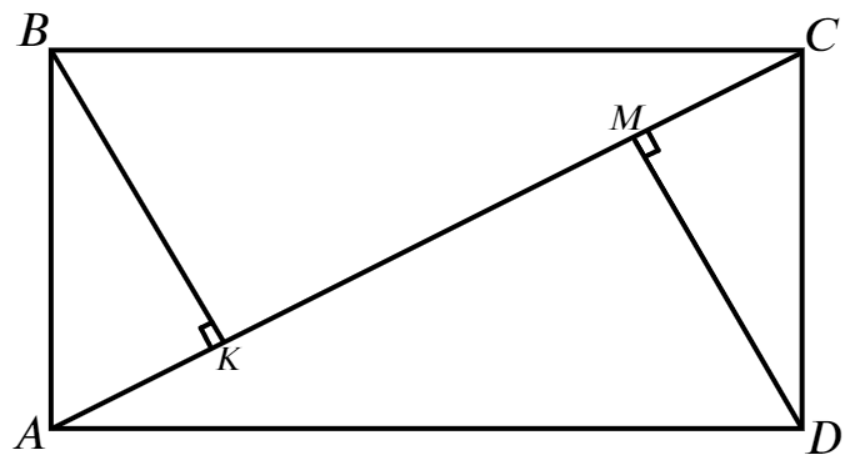
\includegraphics[scale=0.35]{g9-152.png}}
\end{figure}\\
Пусть $AK=CM=x$ (эти отрезки равны так как по катету и гипотенузе равны треугольники $ABK$ и $CDM$). Треугольники $AMD$ и $DMC$ подобны по двум  углам ($\angle AMD=\angle DMC=90^\circ,\ \angle MDC=90^\circ-\angle ACD=\angle CAD).$ Тогда $\cfrac{AM}{MD}=\cfrac{MD}{CM},\ \cfrac{x+5}{6}=\cfrac{6}{x},\ x^2+5x=36,\ x^2+5x-36=0,\
(x-4)(x+9)=0,\ x=4.$ Тогда $S_{ABCD}=2S_{\Delta ACD}=2\cdot\cfrac{1}{2}\cdot6\cdot13=78.$\\
